\chapter{Concepts for Aircraft Manufacturing Automation}
\label{sec:VisionForAircraftManufacturingAutomation}

%%% Citation
\begin{flushright}
{
%\textit{"The problems of the world cannot possibly be solved by skeptics or cynics \\ whose horizons are limited by the obvious realities. We need men who can  \\ dream of things that never were and ask why not?"}
\textit{"We need men who can dream of things that never were and ask why not?"}\\
  -- \emph{John F. Kennedy}
%
%\emph{John F. Kennedy}
}
\end{flushright}
\vspace{+10pt}
%%%%

This chapter presents robotic concepts to automate the manufacturing of airplanes, and discuss challenging actuator requirements motivating the work of this thesis. Automating aircraft production require robots going inside the fuselage, unlike automobile production where the car can be on an assembly line and surrounded by robots. The focus is on the production of commercial aircraft, but discussed issues are relevant in the context of manufacturing any large objects (ships, buildings, etc).

%Additionally, with typically slower rates of production and larger numbers of distinct required operations, 


\section{Current situation}
\label{sec:CurrentSituation}

%Here, the current manufacturing approach and the challenge for automating the manufacturing and assembly of aircraft is briefly explored.
%In the aerospace industry, one technical challenge for the automation of aircraft manufacturing is bringing robots inside the fuselage. 

Currently aircraft manufacturing is dependent on highly qualified manual workers because of the complexity of tasks involved and the difficulty for accessing manufacturing sites. Currently, many temporary assemblies such as scaffolds are used to assist human workers accessing the manufacturing sites. Hence, traditional robotics systems hardly fit this type of environment; industrial robot arms are too heavy and bulky to be used effectively inside the fuselage \cite{parietti_supernumerary_2014} \cite{menon_design_2011}. 

\section{Solution Concepts}

Many concepts have been proposed to address this complex problem. Here, three class of solution are described: long snake-like articulated arms \ref{sec:LightWeightLongManipulatorArm}, wearable robots \ref{sec:WearableRobots} and mobile robots \ref{sec:MobileClimbingRobots}.

\subsection{Light-weight long manipulator arms}
\label{sec:LightWeightLongManipulatorArm}

The first solution is a direct extension of the approach used in the automotive industry: use robotic arms to reach inside the part. However, because of the size of the fuselage and the highly constraint environment, robot arms needs to be very long and highly articulated to be able to reach manufacturing sites. This type of robot arm is usually refer to as snake-like robots \cite{buckingham_r._chitrakaran_v._conkie_r._ferguson_g._et_al._snake-arm_2007}. Fig. \ref{fig:arm_concept} illustrates a concept of a long serial robotic arm reaching inside the fuselage through a window hole.

\begin{figure}[H]
	\centering
		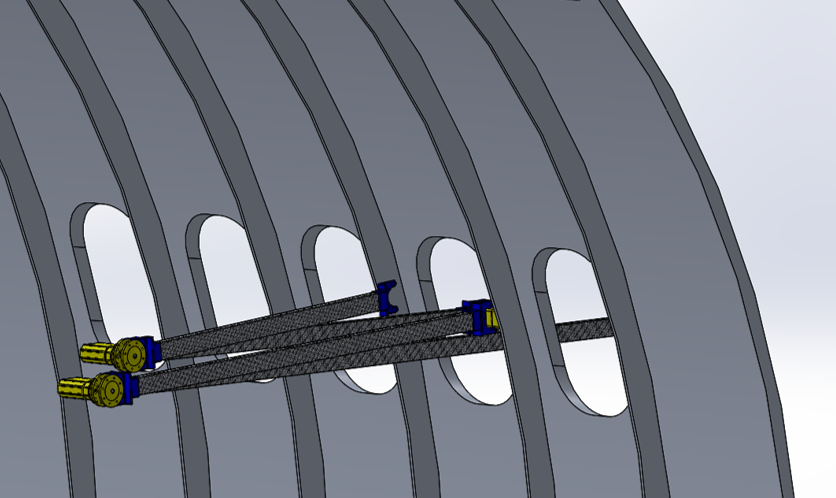
\includegraphics[width=0.9\textwidth]{arm_concept.png}
		\caption{Long light-weight arm concept for interior access}
	\label{fig:arm_concept}
\end{figure}

One of the main bottleneck of such concept is the weight and volume of the actuation system \cite{roy_nonlinear_2009}. With a highly-articulated serial arm, many actuator are required and each of them needs to bear the weight of the payload and posterior links. Moreover, with a highly articulated arms, it is hard to design transmission mechanisms to displace actuators from the joint toward the base of the robot where their weight would be a lesser issue. Hence, typical snake-like arms using electric motor usually struggle just to overcome their own weight and have very limited payload capabilities.


\subsection{Wearable robots}
\label{sec:WearableRobots}

Another possible solution to bring robot on site easily is to use the help of humans, which unlike robot would have no problems navigating and moving inside a manufacturing site. The idea is to augment human capabilities with a wearable robotic system. One approach is using exoskeleton to improve the strengh and precision of worker. An alternative, illustrated at Fig. \ref{fig:wearable_concept}, is super-numary robotic limbs take can be used to brace workers, assist in complex task and others. 

\begin{figure}[H]
	\centering
		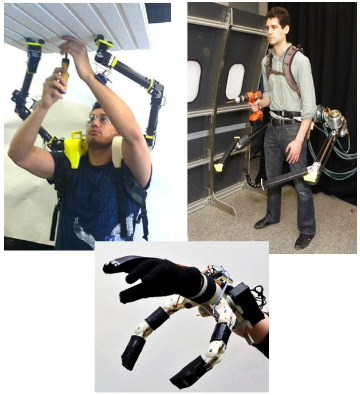
\includegraphics[width=0.6\textwidth]{wearables_robots.png}
		\caption{Wearable robot concepts and prototypes \cite{bonilla_robot_2014} \cite{parietti_supernumerary_2016} \cite{wu_hold-and-manipulate_2015} }
	\label{fig:wearable_concept}
\end{figure}

Because this type of robot are carried by human, weight is also a critical characteristic. It is still a challenge to design wearable robots sufficiently light to be an asset and not a burden to the human wearer.


\subsection{Mobile climbing robots}
\label{sec:MobileClimbingRobots}

Another approach, aiming at a higher level of automation, is to have mobile robots walking or climbing inside the aircraft fuselage to reach manufacturing sites automatically. Fig. \ref{fig:arm_concept} illustrates a spyder-like mobile robot. The idea for this concept is to use local bracing for reaching the force and stiffness required for some manufacturing tasks, and use the same legs for site-to-site locomotion inside the fuselage. 

\begin{figure}[H]
	\centering
		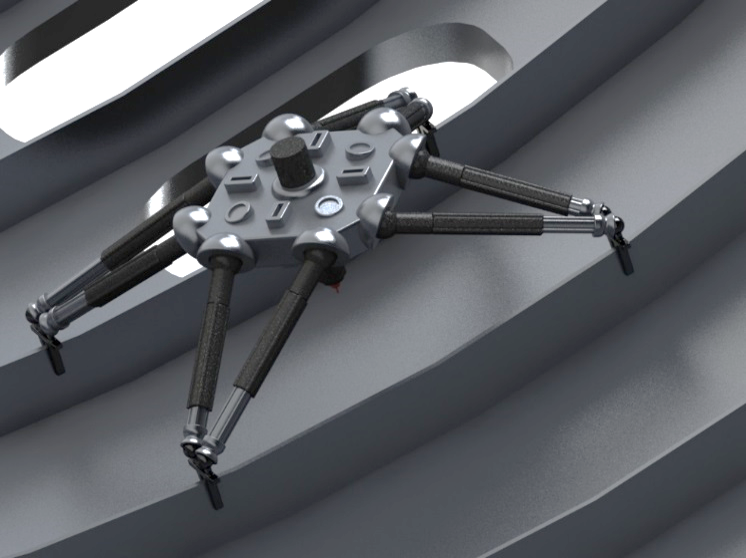
\includegraphics[width=0.8\textwidth]{spyder_concept.png}
		\caption{Mobile climbing manufacturing robot concept}
	\label{fig:climbingrobot}
\end{figure}

\begin{figure}[H]
	\centering
		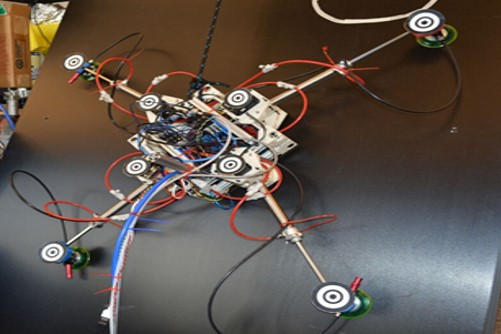
\includegraphics[width=0.8\textwidth]{climbingrobot_proto.jpg}
		\caption{Climbing robot prototype TODO: upload high-quality pic}
	\label{fig:climbingrobot_proto}
\end{figure}

This type of robotic system would face many challenges regarding reaching the required autonomy level. However one fundamental issue is still the weight, since the robot would have to fully bear its own weight as it climbs around the fuselage. Moreover, meeting the requirement of both locomotion and manufacturing tasks with actuators limited in weight and volume is also a challenge. 


\section{Technical challenges}

All those concepts share the same difficulty regarding very challenging actuator requirements. It all comes from the fact for any system that needs to reach manufacturing sites inside a fuselage, volume and weight are highly constrained. Moreover, tasks related to reaching/transportation and manufacturing operations have very different requirement regarding force, speed and impedance. Hence, designing actuation systems meeting a wide-range of requirements, when weight and volume is highly constrained, is not trivial. 

The proposed idea of using robot with actuators equipped with variable transmission directly address those practical challenges limiting many robotic concepts. All the concepts presented in this chapter could hugely benefit from the technology developped in this thesis. 